%^^^^^^^^^^^^^^^^^^^^^^^^^^^^^^^^^^^^^^^^^^^^^^^^^^^^^^^^^^^^^^^^^^^^^^^^^^^^^^^
% La rappresentazione 2D dello spazio delle configurazioni Cinematiche  a supporto compatto
% con aggiunta delle soluzioni della lagrangiana perturbata
%_______________________________________________________________________________

\documentclass{standalone}

%\usetikzlibrary{...}
\usepackage{tikz}
\usepackage{pgfplots}
\pgfplotsset{compat=newest}


\begin{document}
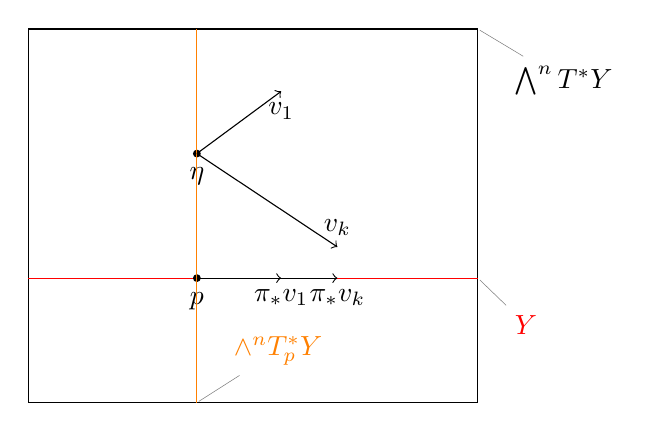
\begin{tikzpicture}
\begin{axis}[axis lines=none,clip=false]

	% Bundle square
	\addplot[color=black] coordinates {
		(8,6) (0,6) (0,0)(8,0)(8,6)
		}node [pos=1,pin={-45:$\bigwedge^n T^\ast Y$},inner sep=0pt] {};

	% Manifold Y Linel
	\addplot[color=red] coordinates {
		(0,2)
		(8,2)
	}node [pos=1,pin={-45:$Y$},inner sep=0pt] {};
	
	% Base point
	\node[label={270:{$p$}},circle,fill,inner sep=1pt] at (axis cs:3,2) {};

	% Bundle point
	\node[label={270:{$\eta$}},circle,fill,inner sep=1pt] at (axis cs:3,4) {};

	% FIber
	\addplot[color=orange] coordinates {
	(3,0)(3,6)
	}node [pos=0,pin={45:$\wedge^n T^\ast_p Y$},inner sep=0pt] {};

           
	%Tangent Vectors to the Bundle
	\addplot[->] coordinates
           {(3,4) (4.5,5)}node [pos=1,label={270:$v_1$},inner sep=0pt] {};	
	\addplot[->] coordinates
           {(3,4) (5.5,2.5)}node [pos=1,label={:$v_k$},inner sep=0pt] {};		
           
	%Projected Vectors 
	\addplot[->] coordinates
           {(3,2) (4.5,2)}node [pos=1,label={270:$\pi_\ast v_1$},inner sep=0pt] {};	
	\addplot[->] coordinates
           {(3,2) (5.5,2)}node [pos=1,label={270:$\pi_\ast v_k$},inner sep=0pt] {};		
	

 \end{axis}
\end{tikzpicture}
\end{document}